%% Fjalar design document
\documentclass{article}
\usepackage{fullpage}
\usepackage{graphicx}
\usepackage{listings}
\usepackage{program}
\usepackage{wrapfig}
\title{Implementation of Fjalar}
\date{}
\author{}
\begin{document} \maketitle
This chapter outlines the implementation of Fjalar, a dynamic analysis
framework for C/C++ programs. 

Fjalar can be broken down into 3 primary modules: The DWARF parser,
which transforms the DWARF information in a program
binary into a more suitable representation, the function
instrumenter, which inserts calls into Fjalar at function entries and
exits of a target program, and the variable traverser, which
collects information about program variables. A diagram of these 3
modules, including their inputs is provided below.

\begin{figure}
\noindent
\centering
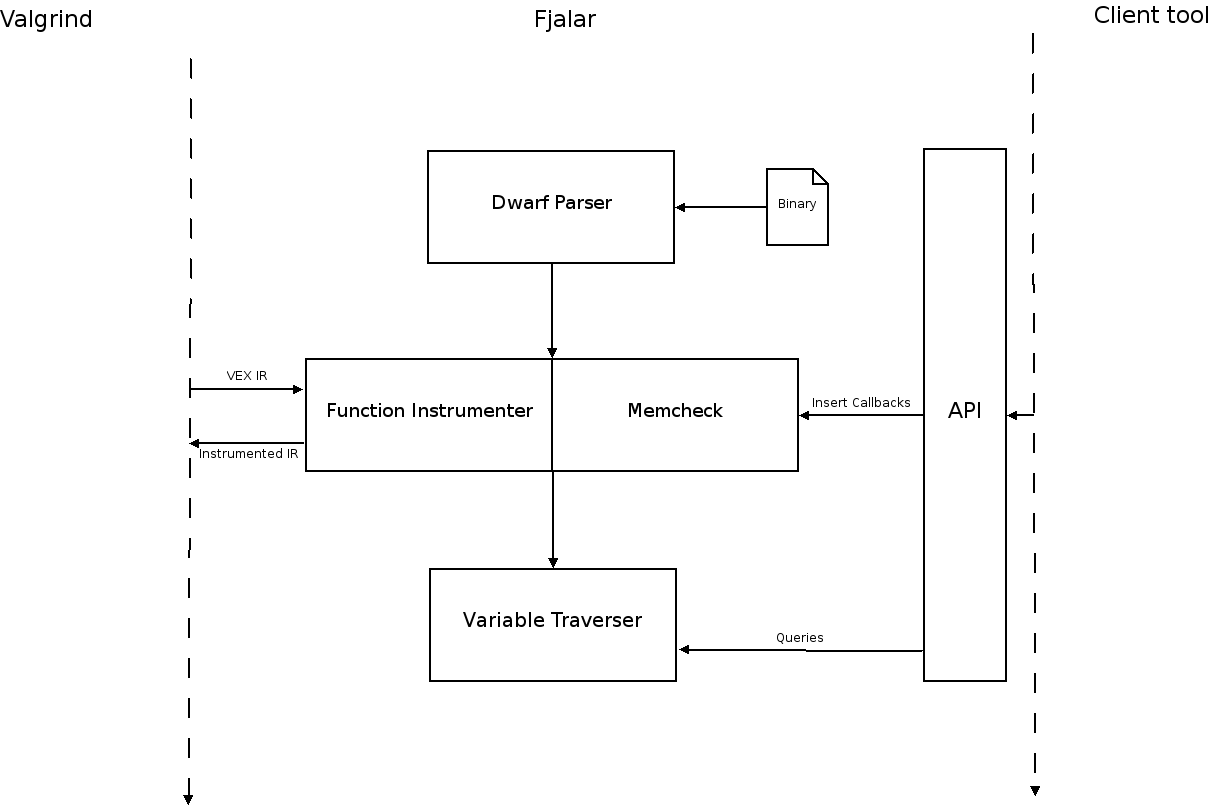
\includegraphics[width=150mm]{fjalar-arch-initial}
\caption{Fjalar architecture}
\end{figure}

This chapter is organized into the following sections: 

\begin{itemize}
\item Section 1 describes Fjalar's DWARF parser
\item Section 2 describes Fjalar's Function instrumenter
\item Section 3 describes Fjalar's Variable traverser
\item Section 4 details Fjalar's API as well as provides an
  implementation of a simple tool
\end{itemize}

\section{The DWARF Parser}
\subsection{The DWARF debugging format}
The purpose of debugging information is to provide a mapping between
the low-level information contained in a binary and the symbolic,
high-level constructs present in the source code. This mapping is
designed to allow debuggers to present higher level to a programmer
than it could otherwise.

DWARF is a standardized format for debugging information
\cite{silverstein1993dwarf}. There are currently 3 versions of the
DWARF format. DWARF version 1 was developed and released in the mid
1980s, but never achieved widespread use due to various inefficiencies.
DWARF version 2 was released in 1993.  The standard was updated again
in 2005 to version 3.  Finally, version 4 was released in 2011.
Version 3 and version 4 are both in use at this time.  Fjalar is
designed to work with DWARF versions 2 through 4.

Fjalar leverages the information available in the DWARF format to
provide an interface for tools to read and modify data in a target
program using source-level constructs.

%**NOTE**: Should I go into depth on the DWARF format

\subsection{Readelf hooks}
Due to the complex nature of both the DWARF debugging information and
the ELF binary format (the standard object file format on Linux),
Fjalar makes use of readelf, a component of GNU Binutils designed to
display information on ELF object files. Fjalar contains a modified
version of readelf in which all the functions for displaying DWARF
information contain callbacks into Fjalar. \texttt{typedata.c} is
responsible for constructing a very low-level, but organized version
of the DWARF information from these callbacks. This low-level 
representation closely mimics the internal structure of the DWARF
information, but is not an appropriate representation for the work
Fjalar does.

\subsection{Translating DWARF information into Fjalar data structures}
The majority of Fjalar's compile-time information is represented by
three data structures: (1) FunctionEntry, (2) VariableEntry, and (3)
TypeEntry. Their declarations can be found in \texttt{fjalar\_include.h}

\subsubsection{FunctionEntry}
The FunctionEntry structure contains information about a particular
function. It contains the function's name, the name of the file in which  
the function is defined, the start and end address of the function's 
instructions, whether or not the function is declared as file-static,
and lists of the function's formal parameters and local variables. 

When dealing with C++ programs, a function's FunctionEntry will also  
contain the mangled and demangled name of the function and, if it's a
member function, a pointer to the TypeEntry of its enclosing class.

\subsubsection{VariableEntry}
The VariableEntry structure contains information about a particular
variable in the program. It contains the name of the variable, whether
it is a global, local, formal parameter, or return variable, the
location of the variable and its declared type. Additionally,
if it is a member variable it contains a pointer to its enclosing
class, struct, or union.

\subsubsection{TypeEntry}
The TypeEntry structure contains information about a particular type used
by the program. There are premade type entries for all the primitive
types defined in C and C++, such as char, int, long, etc.
A TypeEntry contains  the
declared type of the variable, the name of the type, and the size of
the type in bytes.

If the type corresponds to a struct, class, or union (this is referred to
as an aggregate type throughout the Fjalar codebase), it contains a pointer
to an AggregateType structure which contains additional information
including a list of all member variables and, in the case of C++
classes, a list of constructors, destructors, and superclasses.

\subsubsection{Translation}
\texttt{generate\_fjalar\_entries.c} is responsible for translating
the low-level representation that is 
provided by \texttt{typedata.c} into the
data structures defined in section 1.3. It
accomplishes this by taking the representation of the DWARF data and
making 2 passes across it. First it makes a pass for functions. During
this pass Fjalar creates a FunctionEntry for every function contained
in the debugging information and creates 2 hash tables for accessing
them. One hash table is indexed by the address of the function's
starting address (referred to as the startPC), the second is indexed
by the address of the instruction corresponding to the first line of
code (referred to as the entryPC).

Fjalar then makes a second pass over the initial representation,
creating a VariableEntry and, if necessary, a TypeEntry for every
Variable. It is at this point that it associates formal parameters and
local variables with their containing functions, as well as creating a
list of all the global variables in the program.

Finally the function table is iterated over once to make sure that
member functions and constructors/destructors are correctly referenced
by their enclosing class's TypeEntry.

This entire process takes linear time proportional to the size of the
debugging information. This process finishes fairly fast for most
programs, even particularly large C programs. Large C++ programs,
particularly those which make use of templates, are known to contain
large amounts of debugging information \cite{rotithor1999measurement}
and as such will take longer to process.

\section{Function entry and exit handling}
Fjalar instruments the entry and exit of every function in the target
program with a callback into Fjalar. This callback is to allow Fjalar
to collect any information necessary to perform a variable traversal
of the function, which is detailed in section 1.4.2, and to run any
code requested by the client tool.

To perform this instrumentation, Fjalar is built on top of Valgrind, a
framework for dynamic binary instrumentation
\cite{nethercote2007valgrind}. Valgrind was chosen as the basis for
Fjalar's instrumentation functionality due to its ability to work
with unmodified program binaries. Fjalar was designed to be run
on unmodified program binaries with debugging symbols to avoid any
disadvantages of source-based instrumentation or customized
compilation toolchains. This design decision was motivated by
limitations in previous source-based tools encountered when trying to
build a Daikon front-end \cite{Guo2006} (The construction of Kvasir, 
a Daikon front-end built on top of Fjalar is detailed in the following 
chapter).

Valgrind makes use of dynamic binary re-compilation: Valgrind loads a
target program into the same process as itself and then recompiles the
target program's machine code, one small code block at a
time. Valgrind recompiles the machine code block into an intermediate
representation (IR) known as VEX. Valgrind then provides a client tool
with the VEX IR and the ability to instrument the IR with its own VEX
instructions. Valgrind will then translate this instrumented IR block
back into machine code and execute it. This process is covered in much
greater detail in Nethercote \cite{nethercote2007valgrind}.

\subsection{Determining entries and exits}
The DWARF information provides the first and last instructions of a
function, however, this is insufficient for detecting entries and
exits for a few reasons:

For entries, we would prefer to enter after the prologue of the
function has run, as the variable information provided by the DWARF
information tends to only be valid for functions with a valid stack frame.

For exits, the last instruction only corresponds to one possible
exit. For functions with multiple exit points, the compiler
may choose to have multiple instructions which exit the function, so
going by the last instruction is not enough. 

To deal with the above issues Fjalar makes use of both the available DWARF
information and the VEX IR. To determine function entry, Fjalar takes the
startPC, the entryPC (section 1.3.4), and the VEX basic block which
contains the startPC. Fjalar will then examine every instruction
starting from the beginning, asserting it has found an apropriate
entry point if: 

\begin{enumerate}
\item the current instruction is at entryPC, or 
\item if the current instruction is at the end of the basic block. 
\end{enumerate}

The consideration of (2) as a valid entry point is motivated by the
assumption that the prologue will always be completed by the end of
the first basic block of the function. Pseudocode for this algorithm
is provided below.

\begin{program}

\PROC |insert\_entry|(basic\_block) \BODY
  \IF \NOT |contains|(|functionEntryByStartPC|, |basic\_block[0]|) \THEN \EXIT \FI;

   |function| := |get|(functionEntryByStartPC, basic\_block[0]);
   |entryPoint| := |addressOf|(|basic\_block[0]|);

   \FOR |instr| \in |basic\_block| \DO
     \IF |addressOf|(|instr|) \leq f.entryPC \THEN \DO
       |entryPoint| := |addressOf|(|instr|);

   |insert\_call|(|entryPoint|, |FjalarEntryCallBack|)
   \EXIT
   \ENDPROC
 \end{program}

Determining function exits are much simpler due to the Valgrind
representing all functions exits with the VEX IR Statement EXIT. To
instrument function exits, Fjalar just needs to insert callbacks
before every EXIT in the VEX IR.

\subsubsection{Non-local exits}
Non-local exits are particularly troublesome for Fjalar due to the
fact that they do not show up as a normal function exit in the
assembly and accordingly do not show up in the VEX IR as EXIT
statements. Because of this Fjalar will currently not execute exit
instrumentation for any functions that were non-locally exited.

\section{Variable Traversal}
Fjalar provides information about all non-local variables in a
program. This information includes its type, its name, levels of
pointer indirection, and the location of the variable at that point in
the program's execution. Fjalar is able to provide the exact location 
in memory due to Valgrind running its client tools in the same memory
space as the target program.

Due to the memory-unsafe nature of C/C++ safely exploring the
variables in a target C/C++ program is a difficult
proposition and as such, the handling of variable traversal is the
complex aspect of Fjalar. Variables can be broken into 2 groups:
non-pointers and pointers.

For both cases the DWARF information provides us with enough
information to determine the variable's location at run-time.

\subsection{Translating DWARF location information}
Locations in the DWARF information are provided as a sequence of DWARF
expressions. Each DWARF expression is itself made up of a DWARF
operator and one or more DWARF atoms which serve as operands. In
addition to the DWARF atoms the DWARF operations may also perform
operations on an implicit stack. The DWARF location information 
can be thought of as an instruction set for a simple stack machine.

Fjalar currently implements a subset of this instruction set. Fjalar's
DWARF expression interpreter can be found
in\texttt{fjalar\_traversal.c} and complete information about the set
of DWARF operations can be found in Silverstein
\cite{silverstein1993dwarf}.

\subsection{Non-pointer variables}
For these variables, Fjalar simply interprets the sequence of DWARF
expressions in the DWARF information to determine the variable's
address in memory. Variables contained in registers do not need to be treated
specially as Valgrind keeps an in-memory structure of the target
program's register state, and a pointer into this register state is
used as the location of the variable.

\subsection{Pointers and Arrays}
Pointer and array variables give Fjalar the most trouble. The C
language standard does not require that pointers point to a valid
location at all points in the program. Instead it leaves the behavior
of dereferencing pointers which point to invalid locations, such as
NULL or a location that was recently free()'d, as
undefined. This makes Fjalar's job of performing variable traversal
hard. Due to the duality of pointers and arrays in C/C++, the above
also applies to arrays.

\subsubsection{Pointers}
In addition to the variable information mentioned in the previous
section, Fjalar would like to recursively provide the
address in memory of any pointed-to variables. For example In the
following C snippet:

\lstset{language=C, frame=single,}
\begin{lstlisting}
int *ptr1;
int **ptr2;
\end{lstlisting}

Fjalar would like to provide the address of *ptr1, ptr1, **ptr2,
*ptr2, and ptr2. The ptr1 case is relatively trivial because if ptr1
was a properly declared variable, the compiler will have allocated
space somewhere in the program's memory/register space for the
variable (This assumption does not hold in the case of optimized
programs, which Fjalar does not currently support). So in the case of
ptr1 it's simply an issue of providing the address of ptr1, and the
value at that address.

ptr2, however, is much more problematic. ptr2 and *ptr2 are easy for
the same reasons mentioned above. Providing the address of **ptr2,
however, requires Fjalar to examine the  value of *ptr2.
It's worthwhile to examine the
difference in complexity of determining the address of *ptr2 and
**ptr2. It's safe to look up the value of ptr2, as it's an automatic
variable and has been properly
allocated by the compiler, thus finding the address of *ptr2 is easy,
it just requires reading ptr2. The value
in ptr2 may be garbage, however we do not need to actually
dereference this value to provide the address of *ptr2.

Providing the address of **ptr2, however, does require a dereference
of the value ptr2. This is an unsafe operation and could cause both
Fjalar and the target program to crash if ptr2 contains an
invalid memory location. To counteract this Fjalar makes use of
Memcheck, a Valgrind tool designed to detect memory errors 
\cite{nethercote-shadow}. Fjalar queries
Memcheck before accessing any memory location in the target
program, If Memcheck reports the address as either unallocated or
uninitialized Fjalar will not due the dereference and simply mark the
variable as such before passing it to the tool

\subsubsection{Arrays}
The DWARF information gives us some aid in regards to determining the
length of an array. The DWARF information provides us with
size information for arrays allocated on the stack or in global
memory.

This makes it trivial to provide the size for a global array. Arrays
passed as a function argument, however, are more difficult. C does not
support passing an array by value, so when passed to a function,
arrays are decayed into a pointer. To determine whether or not a
pointer argument is an array Fjalar employs the following algorithm to
determine the number of elements a pointer actually points to.

\begin{enumerate}

\item Determine if the address points to the global address space, if so
   try and find a global variable in the DWARF information that could
   correspond to this address. This involves both an equality comparison
   between the address of all variables in the global space, and checking
   if this address is in the bounds of another array.
   
   If a corresponding variable is found, this is a pointer. If this lies
   between the bounds of a global array, this is an array of size
   (END\_ADDR - PTR\_ADDR). 

\item Determine if the address points to a array currently on the stack,
   To do this, Fjalar iterates over all functions currently on the
   stack to try and find one in it's stack frame, Fjalar determines a
   the address range of function's stack frame by subtracting the
   stored stack pointer from the stored frame pointer. If it is in
   some function's stack space, it searches all of the function's
   local variables for a corresponding vaariable with a search
   identical to the 1 proposed in step 1.

\item This step is broken into 2 cases: If the address is in the stack or
  global region, but no corresponding variable is found in previous
  searches, return a size of 1; otherwise continously query memcheck
  for every address from the initial address onwards and return a size
  of(LAST\_INITIALIZED\_ADDRESS - PTR\_ADDR).

\end{enumerate} 
The above algoirthm provides relatively accurate results for stack and
global variables. For heap allocation, however, it tends to
overestimate the size of an array as it is simply returning the
difference between the pointed-to address and the last initialized
element of the dynamically allocated block it belongs to.

\section{Fjalar API}

\subsection{Function instrumentation}
This section describes the function instrumentation portion of the
Fjalar API. Every tool must implement the following 2 functions:

\lstset{language=C, frame=none, basicstyle=\small}
\begin{lstlisting}
void fjalar_tool_handle_function_entrance(FunctionExecutionState*);
void fjalar_tool_handle_function_exit(FunctionExecutionState*);
\end{lstlisting}

Fjalar will insert a call to the first function after the
prologue of every function in the target program, as well as a
call to the second function before every return statement. The
FunctionExecutionState will contain the collected dynamic state of the
target program at the time of the call, including the address of the top of the stack, the
beginning of the current stack frame, and a complete copy of all the
values on the function's stack at entry (this is done to allow
analysis of formal parameters even in situations where the compiler
chooses to use their locations on the stack to store temporaries). 
Additionally it contains a pointer to a FunctionEntry struct (section
1.3.1) which contains the static information known about the function.

Consider the code fragment below:

\lstset{language=C, frame=single,basicstyle=\small}
\begin{lstlisting}
int main(int argc, char **Arv) {
  int b = 5;
  int *p = &b, *q;
  return 5;
}
\end{lstlisting}

Fjalar will instrument the code and insert a call before before the
first instruction of the 'int b = 5', and one more before the last
instruction of the 'return 5'. The behavior of the above function
after instrumentation and translation would be similar to the
behavior following block: 

\begin{lstlisting}
int main(int argc, char **Arv) {
  fjalar_tool_handle_function_entry(state);
  int b = 5;
  int *p = &b, *q;
  fjalar_tool_handle_function_exit(state);
  return 5;
}
\end{lstlisting}


\subsection{Variable Inspection}

Fjalar allows a client tool to inspect all non-local  variables in
scope at a given function entry or exit. This is primarily done
through the following function :

\lstset{language=C, frame=none, basicstyle=\small}
\begin{lstlisting}
void visitVariableGroup();
\end{lstlisting}

The tool provides the variable group to traverse (either global
variables, formal parameters, or the return value), the current top of
the stack (which can be retrieved from the FunctionExecutionState
struct),  and a callback function. Fjalar will then call the callback for every variable within
the group, providing it with a VariableEntry as well as auxiliary
information such as it's location in memory, whether or not it's a
sequence of elements, and the number of elements. Additionally,
Fjalar provides a few convenience functions to examine individual
variables given a VariableEntry, however the information provided is
much more limited as it is unable to determine things like memory
location and number of elements without the run-time information
provided by a FunctionExecutionState.

\subsection{Example Tool}

Below is an example client tool which makes use of the Fjalar API to print
the memory address of all variables at every function entry. Some
trivial functions (such as allocators as well as command line
handlers) are omitted for brevity. A full runnable tool is included in
basic-tool/basic-tool.c 

\lstset{language=C, breakindent=5pt, morecomment=[l][keywordstyle]{//}}
\begin{center}
\begin{lstlisting}
// This simple callback function prints the memory address of a
// program variable
TraversalResult basicAction(VariableEntry* var,
                              char* varName,
                              VariableOrigin varOrigin,
                              UInt numDereferences,
                              UInt layersBeforeBase,
                              Bool overrideIsInit,
                              DisambigOverride disambigOverride,
                              Bool isSequence,
                              // pValue only valid if isSequence is false
                              Addr pValue,
                              Addr pValueGuest,
                              // pValueArray and numElts only valid if
                              // isSequence is true
                              Addr* pValueArray,
                              Addr* pValueArrayGuest,
                              UInt numElts,
                              FunctionEntry* varFuncInfo,
                              Bool isEnter) {
  if (isSequence) {
    VG_(printf)("%s (%p) - %d elements\n" ,varName, pValueArray,  numElts);
  } else {
    VG_(printf)(%s (%p)\n", varName, pValueArray");
  }

  // We want to deref. more pointers so that we can find out array
  // size for derived variables:
  return DEREF_MORE_POINTERS;
}

// These functions are called during every instance of a function
// entrance and exit, respectively:
void fjalar_tool_handle_function_entrance(FunctionExecutionState* f_state) {
  VG_(printf)("[%s - ENTER]\n", f_state->func->fjalar_name);
  
  // Global Variable addresses can be determined without stack
  // information
  VG_(printf)("Global variables:\n");
  visitVariableGroup(GLOBAL_VAR, 0, 1, 0, 0 ,&printAddr);

  VG_(printf)("  Function formal parameters:\n");
  // Pass the necessary stack information to the variable traverser
  visitVariableGroup(FUNCTION_FORMAL_PARAM,
                     f\_state->func,
                     1,
		     (Addr)f_state->virtualStack
		       + f_state->virtualStackFPOffset,
                     f_state->FP,
                     &printAddr);
}

void fjalar_tool_handle_function_exit(FunctionExecutionState* f_state)
{} // Do nothing for exits
\end{lstlisting}
\end{center}

\bibliographystyle{plain}
\bibliography{fjalar}
\end{document}



